
\documentclass[a4paper,11pt]{article}
\usepackage[a4paper, margin=8em]{geometry}

% usa i pacchetti per la scrittura in italiano
\usepackage[french,italian]{babel}
\usepackage[T1]{fontenc}
\usepackage[utf8]{inputenc}
\frenchspacing 

% usa i pacchetti per la formattazione matematica
\usepackage{amsmath, amssymb, amsthm, amsfonts}

% usa altri pacchetti
\usepackage{gensymb}
\usepackage{hyperref}
\usepackage{standalone}

% imposta il titolo
\title{Appunti Elettronica Digitale}
\author{Luca Seggiani}
\date{2026}

% imposta lo stile
% usa helvetica
\usepackage[scaled]{helvet}
% usa palatino
\usepackage{palatino}
% usa un font monospazio guardabile
\usepackage{lmodern}

\renewcommand{\rmdefault}{ppl}
\renewcommand{\sfdefault}{phv}
\renewcommand{\ttdefault}{lmtt}

% disponi il titolo
\makeatletter
\renewcommand{\maketitle} {
	\begin{center} 
		\begin{minipage}[t]{.8\textwidth}
			\textsf{\huge\bfseries \@title} 
		\end{minipage}%
		\begin{minipage}[t]{.2\textwidth}
			\raggedleft \vspace{-1.65em}
			\textsf{\small \@author} \vfill
			\textsf{\small \@date}
		\end{minipage}
		\par
	\end{center}

	\thispagestyle{empty}
	\pagestyle{fancy}
}
\makeatother

% disponi teoremi
\usepackage{tcolorbox}
\newtcolorbox[auto counter, number within=section]{theorem}[2][]{%
	colback=blue!10, 
	colframe=blue!40!black, 
	sharp corners=northwest,
	fonttitle=\sffamily\bfseries, 
	title=~\thetcbcounter: #2, 
	#1
}

% disponi definizioni
\newtcolorbox[auto counter, number within=section]{definition}[2][]{%
	colback=red!10,
	colframe=red!40!black,
	sharp corners=northwest,
	fonttitle=\sffamily\bfseries,
	title=~\thetcbcounter: #2,
	#1
}

% U.D.M
\newcommand{\amp}{\ensuremath{\mathrm{A}}}
\newcommand{\volt}{\ensuremath{\mathrm{V}}}
\newcommand{\meter}{\ensuremath{\mathrm{m}}}
\newcommand{\second}{\ensuremath{\mathrm{s}}}
\newcommand{\farad}{\ensuremath{\mathrm{F}}}
\newcommand{\henry}{\ensuremath{\mathrm{H}}}
\newcommand{\siemens}{\ensuremath{\mathrm{S}}}

% circuiti
\usepackage{circuitikz}
\usetikzlibrary{babel}

% disegni
\usepackage{pgfplots}
\pgfplotsset{width=10cm,compat=1.9}

% disponi codice
\usepackage{listings}
\usepackage[table]{xcolor}

\definecolor{codegreen}{rgb}{0,0.6,0}
\definecolor{codegray}{rgb}{0.5,0.5,0.5}
\definecolor{codepurple}{rgb}{0.58,0,0.82}
\definecolor{backcolour}{rgb}{0.95,0.95,0.92}

\lstdefinestyle{codestyle}{
		backgroundcolor=\color{black!5}, 
		commentstyle=\color{codegreen},
		keywordstyle=\bfseries\color{magenta},
		numberstyle=\sffamily\tiny\color{black!60},
		stringstyle=\color{green!50!black},
		basicstyle=\ttfamily\footnotesize,
		breakatwhitespace=false,         
		breaklines=true,                 
		captionpos=b,                    
		keepspaces=true,                 
		numbers=left,                    
		numbersep=5pt,                  
		showspaces=false,                
		showstringspaces=false,
		showtabs=false,                  
		tabsize=2
}

\lstdefinestyle{shellstyle}{
		backgroundcolor=\color{black!5}, 
		basicstyle=\ttfamily\footnotesize\color{black}, 
		commentstyle=\color{black}, 
		keywordstyle=\color{black},
		numberstyle=\color{black!5},
		stringstyle=\color{black}, 
		showspaces=false,
		showstringspaces=false, 
		showtabs=false, 
		tabsize=2, 
		numbers=none, 
		breaklines=true
}

\lstdefinelanguage{javascript}{
	keywords={typeof, new, true, false, catch, function, return, null, catch, switch, var, if, in, while, do, else, case, break},
	keywordstyle=\color{blue}\bfseries,
	ndkeywords={class, export, boolean, throw, implements, import, this},
	ndkeywordstyle=\color{darkgray}\bfseries,
	identifierstyle=\color{black},
	sensitive=false,
	comment=[l]{//},
	morecomment=[s]{/*}{*/},
	commentstyle=\color{purple}\ttfamily,
	stringstyle=\color{red}\ttfamily,
	morestring=[b]',
	morestring=[b]"
}

% disponi sezioni
\usepackage{titlesec}

\titleformat{\section}
	{\sffamily\Large\bfseries} 
	{\thesection}{1em}{} 
\titleformat{\subsection}
	{\sffamily\large\bfseries}   
	{\thesubsection}{1em}{} 
\titleformat{\subsubsection}
	{\sffamily\normalsize\bfseries} 
	{\thesubsubsection}{1em}{}

% disponi alberi
\usepackage{forest}

\forestset{
	rectstyle/.style={
		for tree={rectangle,draw,font=\large\sffamily}
	},
	roundstyle/.style={
		for tree={circle,draw,font=\large}
	}
}

% disponi algoritmi
\usepackage{algorithm}
\usepackage{algorithmic}
\makeatletter
\renewcommand{\ALG@name}{Algoritmo}
\makeatother

% disponi numeri di pagina
\usepackage{fancyhdr}
\fancyhf{} 
\fancyfoot[L]{\sffamily{\thepage}}

\makeatletter
\fancyhead[L]{\raisebox{1ex}[0pt][0pt]{\sffamily{\@title \ \@date}}} 
\fancyhead[R]{\raisebox{1ex}[0pt][0pt]{\sffamily{\@author}}}
\makeatother

\begin{document}
% sezione (data)
\section{Lezione del 17-04-26}

% stili pagina
\thispagestyle{empty}
\pagestyle{fancy}

% testo
Nelle scorse lezioni abbiamo visto i transistor MOSFET a canale N, cioè che funzionavano formando un canale di elettroni liberi per la conduzione di elettroni da drain a source. Avevamo detto che questi entravano in conduzione per tensione di gate $V_{GS} \geq V_T$ tensione di threshold. Chiamiamo questi mosfet anche \textbf{NMOS} (\textit{Negative Metal Oxide Semiconductor}), appunto per il fatto che si basano su un canale di portatori negativi (di tipo N).

\subsubsection{Modulazione di canale}
Avevamo detto che in regione di \textit{saturazione} (che è quella che ci interessava per la logica digitale), la corrente nel MOSFET fra source e drain era determinata da:
$$
i_{ds} = \mu_n C_{ox} \frac{W}{L} \frac{ (V_{GS} - V_T)^2 }{2} = K (V_{GS} - V_T)^2
$$
che dava una caratteristica di uscita simile a quella del BJT. Come per il BJT, notiamo che la dipendenza è leggermente lineare all'aumentare di $V_{DS}$, presentando un effetto simile all'effetto di \textit{Early} (visto in 10.1.5). Chiamiamo questo effetto \textit{modulazione di canale}.

La modulazione di canale è determinata dal fatto che le caratteristiche assunte costanti nella lezione 15, e in particolare la lunghezza $\Delta L$ della giunzione PN formata dapo il punto di pinchoff, non portano a conduzione effettivamente costante ma che cresce leggermente al crescere della tensione applicata.

Possiamo modellizzare questo effetto introducendo un termine dipendente da $V_{DS}$ nella caratteristica di uscita in saturazione:
$$
i_{ds} = \mu_n C_{ox} \frac{W}{L} \frac{ (V_{GS} - V_T)^2 }{2} = K (V_{GS} - V_T)^2 (1 + \lambda v_{DS})
$$
Notiamo quindi che, per $\Delta L >> L$ larghezza del canale, le caratteristiche di uscita formano un fascio di rette che passano per l'ascissa $-\frac{1}{\lambda}$, come avevamo visto per l'effetto di Early.

In ogni caso, come avevamo fatto nei BJT, trascureremo l'effetto modulazione di campo nei MOSFET (a volte detto \textit{effetto Early dei MOSFET}) nei circuiti che studieremo.

\subsubsection{Curva transcaratteristica}

\subsubsection{MOSFET a canale P}
Finora abbiamo visto il MOSFET a canale N. Ne esiste un duale, che è il mosfet a \textbf{canale P}. Questo è disposto esattamente al contrario del MOSFET di tipo N, cioè è realizzato su un substrato di tipo N, e ha nodi source, e drain di tipo P.

\begin{center}
	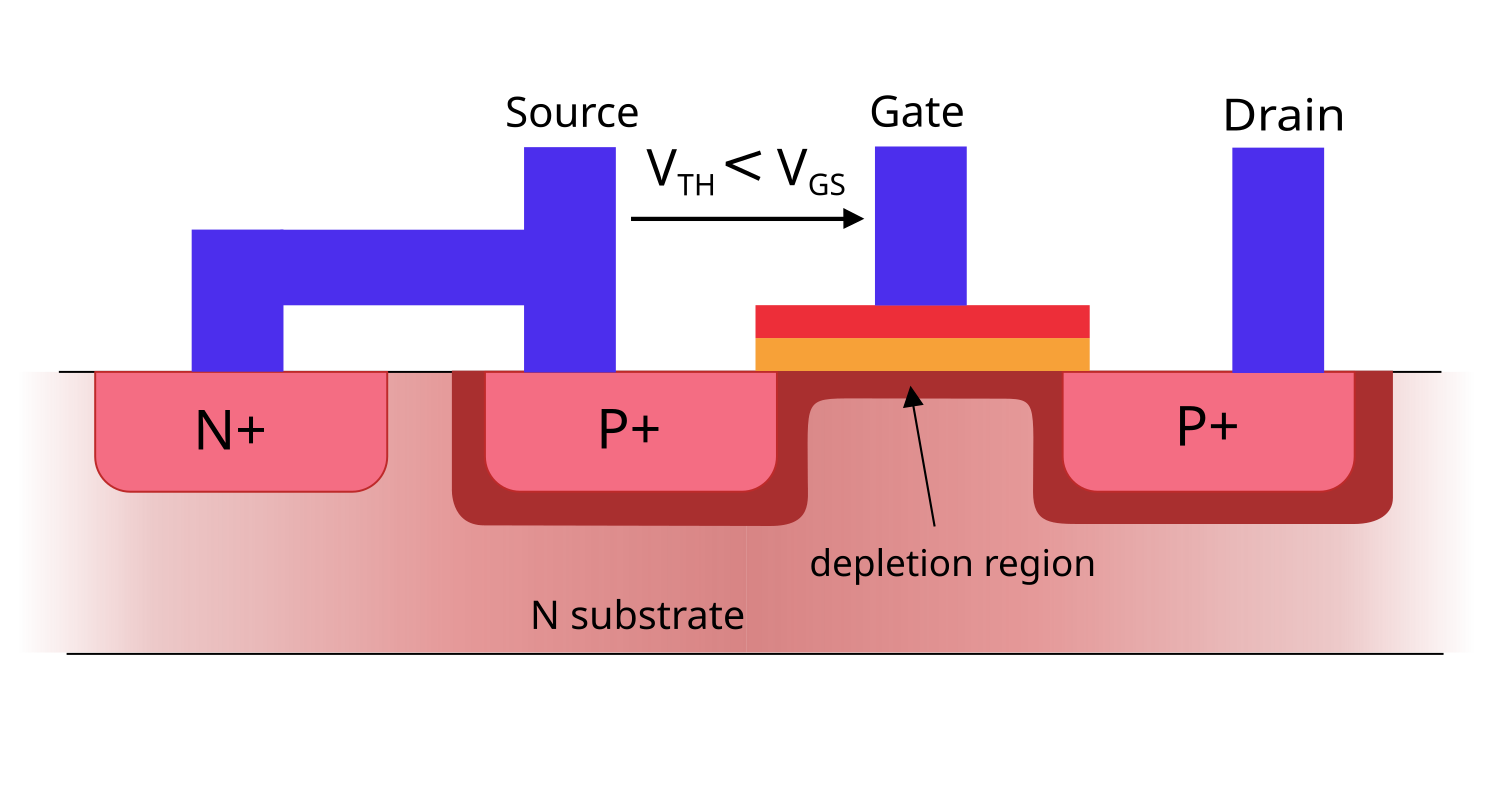
\includegraphics[scale=1]{../figures/mosfet_p.png}
\end{center}

L'idea è di creare un canale di conduttori P fra source e drain, imponendo una tensione negativa al gate. 

Come era stato fra NPN e PNP, il MOSFET a canale P (\textit{PMOS}) è l'esatto duale del MOSFET a canale N, per cui si hanno tutti gli stessi valori, ma cambiati di segno.
Ad esempio:
\begin{itemize}
	\item La $V_T$ del PMOS, che chiamiamo $V_{TP}$, sarà negativa in quanto il gate dovrà attirare verso l'alto le lacune nel substrato N. Avremo quindi:
$$
V_T \leq 0
$$
	\item La $V_{GS}$ dovrà anch'essa essere negativa (per le stesse motivazioni di cui sopra). Ne segue che il senso della disuguaglianza per la condizione è rovesciato:
$$
V_{GS} \leq V_{TP}
$$
\item Anche la tensione fra source e drain sarà invertita ($V_{DS} < 0$), in quanto i portatori di carica saranno le lacune, e quindi lo spostamento delle cariche sarà concorde alla direzione della corrente convenzionale.
\end{itemize}

La caratteristica di saturazione del PMOS sarà quindi analoga, ma con segno invertito, a quella del NMOS:
$$
i_{SD} = \mu_P C_{ox} \frac{W}{L} \frac{(V_{GS} - V_{TP})^2}{2}
$$
con alcune differenze che però vanno notate:
\begin{enumerate}
	\item Innanzitutto consideriamo $\mu_P$ anziché $\mu_N$, che abbiamo detto più volte è più piccola (le lacune sono in genere meno mobili degli elettroni);
\item C'è anche una differenza, in generale, fra le tensioni di threshold $V_{TN}$ e $V_{TP}$. 

	Esistono dei processi (che abbiamo già anticipati) detti \textbf{CMOS} (\textit{Complementary Metal Oxide Semiconductor}). Nei processi CMOS si usano paia complementari di PMOS e NMOS per effettuare funzioni logiche. In questo contesto dobbiamo avere MOSFET di entrambi i tipi che siano \textit{effettivamente} complementari, cioè abbiano caratteristiche invertite ma uguali in modulo. 
\end{enumerate}

\subsubsection{Simboli circuitali del MOSFET}
Viste le varie tipologie, e la vasta gamma di applicazione, dei MOSFET, si ha una serie di simboli che vengono usati per rappresentarli nei circuiti.

\begin{center}
	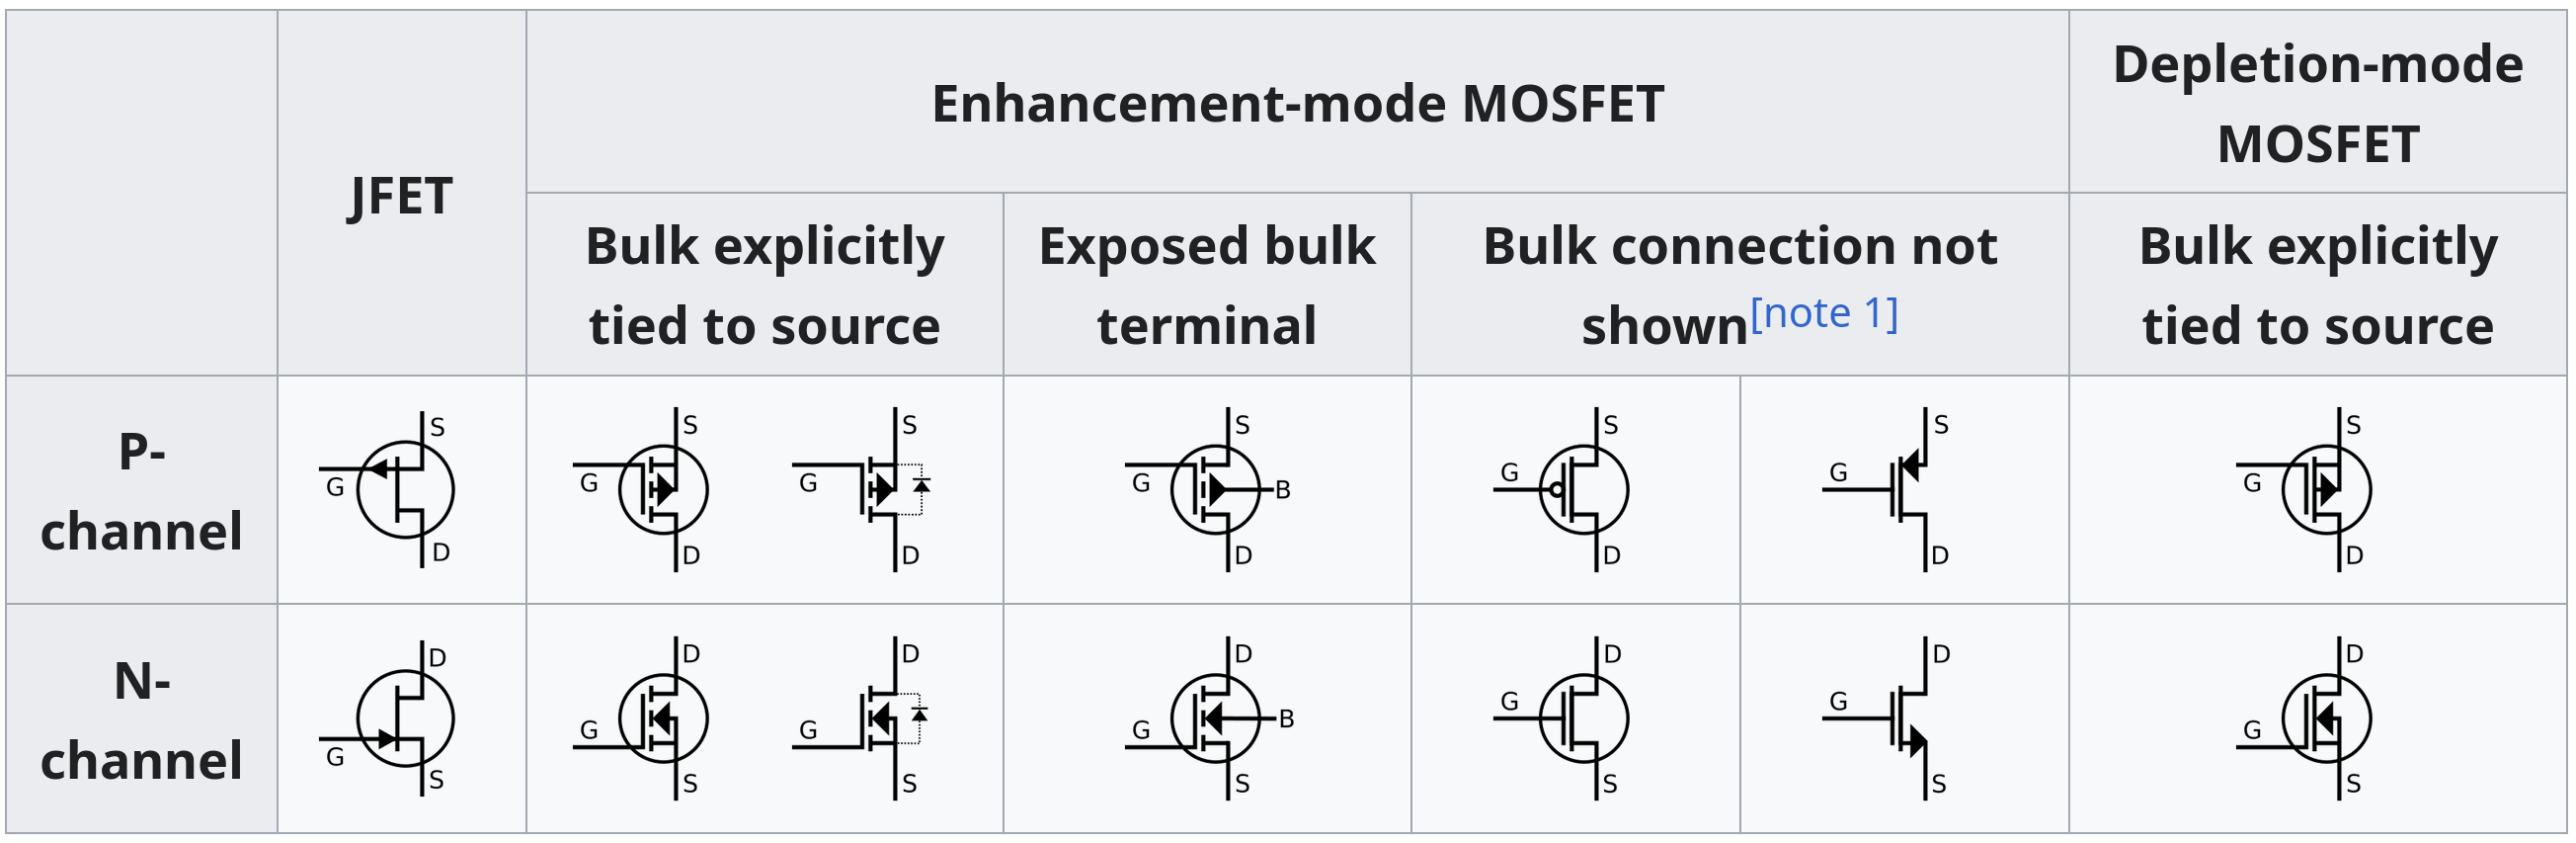
\includegraphics[scale=0.16]{../figures/mosfet_sym.png}
\end{center}

\begin{itemize}
	\item 
Solitamente la rappresentazione con la freccia che indica la direzione della corrente (quella a destra nella colonna \textit{"Bulk connection not shown"}) viene usata nei circuiti analogici;
	\item
La rappresentazione senza freccia, e che distingue il PMOS con il pallino (quella a sinistra nella colonna \textit{"Bulk connection not shown"}), viene invece usata nei circuiti digitali;
	\item 
Nei circuiti discreti, solitamente si usano MOSFET in package che già uniscono il morsetto body al morsetto source. Nei circuiti integrati, invece, il body è presente e si usano i simboli nella colonna \textit{"Exposed bulk terminal"}.
\end{itemize}

Notiamo quindi che esistono altre tipologie di MOSFET che non abbiamo trattato, come i MOSFET a \textit{svuotamento} e ad \textit{arricchimento}, dove il costruttore ha giù ricavato un canale di conduzione che possiamo allargare o restringere a piacimento modulando la tensione di gate.

\subsection{Modelli per il MOSFET}
Iniziamo quindi a vedere i modelli che usiamo per approssimare il comportamento dei MOSFET, a partire dal modello ai \textit{grandi segnali}.
\begin{itemize}
	\item Per l'ipotesi di \textbf{saturazione}, abbiamo che il MOSFET si comporta da generatore di corrente controllato in tensione che obbedisce a:
$$
I_{DS} = K\frac{(V_{GS} - V_T)^2}{2}
$$
La resistenza fra gate e source viene posta ad infinito, e quindi il gate si comporta come un polo isolato.

Vediamo il circuito per un NMOS, dove la corrente va da source a drain:
% circuito

Il PMOS è equivalente, ma con la corrente che va da drain a source:
% circuito

La \textit{verifica} in questo caso si fa ponendo di trovarsi in zona di saturazione, cioè che sia rispettata:
$$
V_{DS} \geq (V_{GS} - V_T)
$$
nel NMOS, e:
$$
V_{DS} \leq (V_{GS} - V_T)
$$
nel PMOS (con tutti i parametri $< 0$).

\item Per l'ipotesi di regione \textbf{ohmica}, abbiamo che il MOSFET si comporta ancora da generatore di corrente controllato in tensione che obbedisce a:
$$
I_{DS} = K\frac{(V_{GS} - V_T)^2}{2}
$$
La resistenza fra gate e source viene posta ad infinito, e quindi il gate si comporta ancora come un polo isolato.

Vediamo il circuito per un NMOS, dove la corrente va da source a drain:
% circuito

Il PMOS è equivalente, ma con la corrente che va da drain a source:
% circuito

La \textit{verifica} in questo caso si fa ponendo di trovarsi in zona ohmica, cioè che sia rispettata:
$$
V_{DS} < (V_{GS} - V_T)
$$
nel NMOS, e:
$$
V_{DS} < (V_{GS} - V_T)
$$
nel PMOS (con tutti i parametri $< 0$).

\end{itemize}

\subsubsection{Circuito di polarizzazione del MOSFET}
Vediamo quindi come si possono creare reti di polarizzazione per far lavorare un MOSFET nella regione di saturazione.

\par\smallskip

\noindent
\textbf{\textsf{Rete a 3 resistori}}

\noindent
Potremmo pensare come primo circuito la classica rete a 3 resistenze con punto di bias dal $V_{cc}$:
\begin{center}
\begin{circuitikz}
\ctikzset{tripoles/mos style/arrows}
\draw
(0,0) node[ground]{} to[R=$R_2$] (0,3)
to[R=$R_1$] (0,6) node[vcc]{};

\draw (0,3) -- (2,3);

\draw (2,3) node[nmos, anchor=B] (Q1) {};

\draw (Q1.C) to[R=$R_D$] ++(0,3) node[vcc]{};
\draw (Q1.E) to[short] ++(0,-3) node[ground]{};

\draw[->] (1.2,3.3) -- (1.8,3.3) node[midway, above]{$I_G$};
\draw[->] (Q1.C) ++(0.3,0.5) -- ++(0,-1) node[midway, right]{$I_D$};
\draw[->] (Q1.E) ++(0.3,0) -- ++(0,-.8) node[midway, right]{$I_S$};

\end{circuitikz}
\end{center}

In questo circuito la rete a sinistra (formata da $R_1$ e $R_2$) fa da partitore di tensione se la corrente $I_G = 0$ è nulla. In tal caso vale:
$$
V_G = V_{cc} \frac{R_2}{R_1 + R_2} = V_{GS}
$$
in quanto $V_S = 0$ (è direttamente collegata al ground).

Se la corrente $I_G$ è 0, per il MOSFET (che è un tripolo) dovrà valere:
$$
I_G = 0 \implies I_D = I_S
$$
e quindi:
$$
V_{cc} = R_D I_D + V_{DS}
$$
Abbiamo allora una retta di lavoro sul grafico tensione-corrente:
$$
I_D = \frac{V_{cc}}{R_D} - \frac{V_{DS}}{R_D}
$$
che sfruttando il modello analitico porta al sistema per il punto di quiescenza:
$$
\begin{cases}
I_D = \frac{V_{cc}}{R_D} - \frac{V_{DS}}{R_D} \\
I_D = K \frac{(V_{GS} - V_T)^2}{2}
\end{cases}
$$

\par\smallskip

\noindent
\textbf{\textsf{Rete a 4 resistori}}

\noindent
Una problematica della scorsa rete è che, al variare delle caratteristiche del MOSFET, si possono avere delle varazioni della caratteristica e quindi diverse intersezioni sulla retta di calcolo. Un modo per stabilizzare questa situazione è quello di introdurre una resistenza al source, quindi realizzare una rete a 4 resistori.
\begin{center}
\begin{circuitikz}
\ctikzset{tripoles/mos style/arrows}
\draw
(0,0) node[ground]{} to[R=$R_2$] (0,3)
to[R=$R_1$] (0,6) node[vcc]{};

\draw (0,3) -- (2,3);

\draw (2,3) node[nmos, anchor=B] (Q1) {};

\draw (Q1.C) to[R=$R_D$] ++(0,3) node[vcc]{};
\draw (Q1.E) to[R=$R_S$] ++(0,-3) node[ground]{};

\draw[->] (1.2,3.3) -- (1.8,3.3) node[midway, above]{$I_G$};
\draw[->] (Q1.C) ++(0.3,0.5) -- ++(0,-1) node[midway, right]{$I_D$};
\draw[->] (Q1.E) ++(0.3,0) -- ++(0,-.8) node[midway, right]{$I_S$};

\end{circuitikz}
\end{center}

In questo caso avremo, che, con le stesse ipotesi di prima, la rete a sinistra fa da partitore:
$$
V_G = V_{cc} \frac{R_2}{R_1 + R_2} = V_{GS}
$$
A cambiare sarà la $V_{GS}$, in quanto il source non sarà più direttamente connesso al ground, ma presenterà una caduta su $R_S$:
$$
V_S = R_S I_S = R_S I_D
$$
sempre dal fatto che con $I_G = 0$, $I_D = I_S$ (tripolo), per cui:
$$
V_{GS} = V_G - V_S = V_{cc}\frac{R_2}{R_1 + R_2} - R_S I_D
$$

Notiamo quindi di aver ottenuto una retta per la tensione fra gate e source $V_{GS}$ che dipende da un certo parametro $\alpha$:
$$
V_{GS} = \alpha - R_S I_D, \quad \alpha = V_{cc}\frac{R_2}{R_1 + R_2}
$$
notiamo che questa interseca la corrente nulla in $\alpha$, e la tensione nulla in $\frac{\alpha}{R_S}$, per cui variando $R_S$ possiamo stabilizzare il punto di quiescenza della $V_S$ e il regime di operazione del MOSFET, anche al variare delle sue caratteristiche.

Continuando a risolvere il circuito, possiamo scrivere come prima $V_{cc}$ in funzione per trovare la retta di carico:
$$
V_{cc} = R_D I_D + V_{DS} + R_S I_D = (R_D + R_S) I_D + V_{DS}
$$
Abbiamo allora anche qui una retta di lavoro sul grafico tensione corrente:
$$
I_D = \frac{V_{cc}}{R_D + R_S} - \frac{V_{DS}}{R_D + R_S}
$$
Mettiamo quindi la retta di lavoro a sistema con la caratteristica del MOSFET, dove possiamo sostituire l'equazione per la $V_{GS}$ trovata prima:
$$
\begin{cases}
	I_D = \frac{V_{cc}}{R_D + R_S} - \frac{V_{DS}}{R_D + R_S} \\
	I_D = K \frac{(V_{GS} - V_T)^2}{2}
\end{cases}
\rightarrow
\begin{cases}
	I_D = \frac{V_{cc}}{R_D + R_S} - \frac{V_{DS}}{R_D + R_S} \\
	I_D = K \frac{(\alpha - R_S I_D - V_T)^2}{2}
\end{cases}
$$

\end{document}
